\chapter{动态规划 (Dynamic programming)}

在前几章中，我们见识了一些优雅的算法设计原则——例如分治、图遍历以及贪心选择——它们为一系列重要的计算任务带来了决定性的最优算法。但这些工具的局限在于：它们只能应用于非常特定类型的问题。现在，我们转向算法工具箱中的两大重型武器：\textbf{动态规划 (Dynamic programming)} 与 \textbf{线性规划 (Linear programming)}。当更专门的方法无能为力时，可以借助这两种具有极其广泛适用性的通用技术。不出所料，这种高度的通用性往往以一定的计算效率为代价。

\section{重访 DAG 中的最短路径 (Shortest paths in dags, revisited)}

在第 4 章结束对最短路径的研究时，我们观察到该问题在有向无环图（DAG）中格外简单。让我们重新审视这一情形，因为\textbf{它构成了动态规划的核心灵魂}。

DAG 的独特标志性特征在于其节点可以被\textbf{线性化}（拓扑排序）：即它们可以排在一条直线上，使得所有的有向边都严格从左指向右（图 6.1）。为了理解这为何对最短路径有巨大帮助，假设我们要计算从源点 $S$ 到其他所有节点的距离。具体而言，聚焦于节点 $D$：到达 $D$ 的唯一途径是经过它的前驱节点 $B$ 或 $C$。因此要找到到达 $D$ 的最短路径，只需比较这两条路线：
\[
\text{dist}(D) = \min\{\text{dist}(B) + 1,\; \text{dist}(C) + 3\}.
\]
对于图中的每一个节点都可以写出类似的递推关系。如果我们按照图 6.1 中从左到右的拓扑顺序依次计算这些 $\text{dist}$ 值，就可以完全确信：当我们处理到某个节点 $v$ 时，计算 $\text{dist}(v)$ 所需的全部前驱信息早已被计算就绪。因此只需单趟遍历即可求出所有距离：

\begin{algorithmic}[1]
\State 将所有 $\text{dist}(\cdot)$ 初始化为 $\infty$
\State $\text{dist}(s) = 0$
\For{每个 $v \in V \setminus \{s\}$（按照拓扑线性化顺序）}
    \State $\text{dist}(v) = \min_{(u, v) \in E} \{\text{dist}(u) + l(u, v)\}$
\EndFor
\end{algorithmic}

注意该算法本质上是在求解一组子问题集合 $\{\text{dist}(u) : u \in V\}$。我们从最小的子问题 $\text{dist}(s)$ 开始（已知其答案为 0），随后依次推进到越来越“大”的子问题——即拓扑序列中越来越靠后的顶点的距离。

\begin{figure}[htbp]
\centering
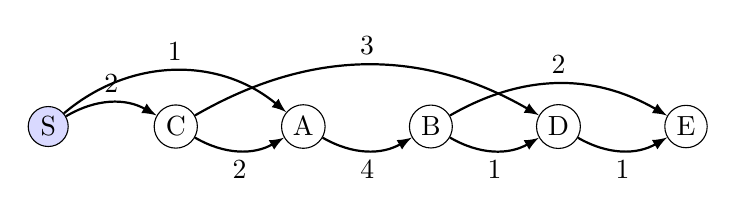
\begin{tikzpicture}[scale=0.9, auto, >=latex]
    \node[circle,draw,fill=blue!15,inner sep=2pt] (S) at (0,0) {S};
    \node[circle,draw,inner sep=2pt] (C) at (1.8,0) {C};
    \node[circle,draw,inner sep=2pt] (A) at (3.6,0) {A};
    \node[circle,draw,inner sep=2pt] (B) at (5.4,0) {B};
    \node[circle,draw,inner sep=2pt] (D) at (7.2,0) {D};
    \node[circle,draw,inner sep=2pt] (E) at (9.0,0) {E};

    \draw[->,thick] (S) to[bend left=30] node[above] {2} (C);
    \draw[->,thick] (S) to[bend left=40] node[above] {1} (A);
    \draw[->,thick] (C) to[bend right=30] node[below] {2} (A);
    \draw[->,thick] (C) to[bend left=30] node[above] {3} (D);
    \draw[->,thick] (A) to[bend right=30] node[below] {4} (B);
    \draw[->,thick] (B) to[bend right=30] node[below] {1} (D);
    \draw[->,thick] (B) to[bend left=30] node[above] {2} (E);
    \draw[->,thick] (D) to[bend right=30] node[below] {1} (E);
\end{tikzpicture}
\caption{线性化拓扑序列上的 DAG 与子问题单向依赖}
\label{fig:dag_dp_linear}
\end{figure}

这是一项极其通用的技术。在每个节点处，我们计算其所有前驱节点值的某种函数。如果将求最小值改为求最大值，就能求出 DAG 中的最长路径；如果将求和改为求积，就能求出边权乘积最小的路径。

\textbf{动态规划}是一种极为强大的算法范式：它通过明确定义一组子问题，并从小到大逐一解决它们；利用较小子问题的答案来帮助求解较大的子问题，直到整个问题最终得到解决。在动态规划中，输入中往往并没有显式给出 DAG；\textbf{DAG 是隐式的}。它的节点是我们定义的各个子问题，它的有向边是子问题之间的依赖关系：若求解子问题 $B$ 需要子问题 $A$ 的答案，则存在一条从 $A$ 到 $B$ 的概念有向边。

\section{最长递增子序列 (Longest increasing subsequences)}

在最长递增子序列（LIS）问题中，输入是一个数字序列 $a_1, a_2, \dots, a_n$。子序列是指按原始顺序选取的任意子集 $a_{i_1}, a_{i_2}, \dots, a_{i_k}$（其中 $1 \le i_1 < i_2 < \dots < i_k \le n$），递增子序列要求其中的数字严格单调递增。目标是找到长度最大的递增子序列。例如序列 $5, 2, 8, 6, 3, 6, 9, 7$ 的最长递增子序列为 $2, 3, 6, 9$（长度为 4）。

为了构建解空间，我们为每个元素 $a_i$ 建立一个节点 $i$，若 $i < j$ 且 $a_i < a_j$，则连一条有向边 $(i, j)$（图 6.2）。
注意到：(1) 该图是一个 DAG；(2) 递增子序列与该 DAG 中的有向路径一一对应。因此，问题转化为\textbf{在该 DAG 中寻找最长路径}！

\begin{figure}[htbp]
\centering
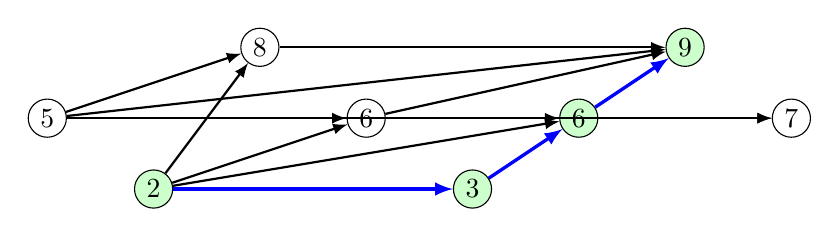
\begin{tikzpicture}[scale=0.9, auto, >=latex]
    \node[circle,draw,inner sep=2pt] (1) at (0,1) {5};
    \node[circle,draw,fill=green!20,inner sep=2pt] (2) at (1.5,0) {2};
    \node[circle,draw,inner sep=2pt] (3) at (3,2) {8};
    \node[circle,draw,inner sep=2pt] (4) at (4.5,1) {6};
    \node[circle,draw,fill=green!20,inner sep=2pt] (5) at (6,0) {3};
    \node[circle,draw,fill=green!20,inner sep=2pt] (6) at (7.5,1) {6};
    \node[circle,draw,fill=green!20,inner sep=2pt] (7) at (9,2) {9};
    \node[circle,draw,inner sep=2pt] (8) at (10.5,1) {7};

    \draw[->,thick] (1)--(3); \draw[->,thick] (1)--(4); \draw[->,thick] (1)--(6); \draw[->,thick] (1)--(7); \draw[->,thick] (1)--(8);
    \draw[->,very thick,blue] (2)--(5); \draw[->,thick] (2)--(3); \draw[->,thick] (2)--(4); \draw[->,thick] (2)--(6);
    \draw[->,very thick,blue] (5)--(6); \draw[->,very thick,blue] (6)--(7); \draw[->,thick] (4)--(7); \draw[->,thick] (3)--(7);
    \draw[->,thick] (6)--(8);
\end{tikzpicture}
\caption{递增子序列构成的隐式 DAG（蓝色加粗路径为最优解 $2 \to 3 \to 6 \to 9$）}
\label{fig:lis_dag}
\end{figure}

定义子问题：令 $L(j)$ 为以第 $j$ 个元素 $a_j$ 结尾的最长递增子序列的长度。
递推状态转移方程为：
\[
L(j) = 1 + \max \{L(i) : (i, j) \in E\} = 1 + \max \{L(i) : i < j \text{ 且 } a_i < a_j\}.
\]
最终全局最优解即为 $\max_{1 \le j \le n} L(j)$。
算法通过双重循环实现，总时间复杂度为 $O(n^2)$。通过维护前驱指针 $\text{prev}(j)$，可以在求出最大值后回溯重构出最优子序列本身。

\begin{sidebarbox}{递归？不，谢谢！ (Recursion? No, thanks.)}
$L(j)$ 的递推式同样提示了一种纯递归算法。但递归在此处是极其灾难性的：其运行时间将达到指数级！原因在于递归过程中没有记忆能力，导致大量相同的子问题被反反复复重复计算。

分治算法之所以能够高效使用递归，是因为分治将问题规模大幅削减（例如减半）；而动态规划中的子问题通常仅比原问题小一点点（例如从 $j$ 到 $j - 1$），导致递归树拥有多项式深度与指数级节点数。动态规划通过\textbf{显式列举所有子问题并按自底向上的顺序一次性求解并记录结果}，从而彻底消除了重复计算。
\end{sidebarbox}

\begin{sidebarbox}{编程（Programming）一词的词源}
“动态规划”（Dynamic programming）中“programming”一词的由来与编写计算机代码几乎毫无关系。它最早由理查德·贝尔曼（Richard Bellman）在 20 世纪 50 年代提出，当时计算机编程还是一项极为小众的技术。在那个时代，programming 指的是“规划、制定计划日程”，而动态规划最初是用来对多阶段决策过程进行最优规划的数学方法。
\end{sidebarbox}

\section{编辑距离 (Edit distance)}

当拼写检查器遇到可能的拼写错误时，会在字典中查找与之最接近的单词。两个字符串之间的相似度可以通过它们之间的\textbf{对齐 (alignment)} 程度来衡量：

\begin{center}
\begin{tabular}{ccccccc}
S & - & N & O & W & Y \\
S & U & N & N & - & Y
\end{tabular}
\quad (代价: 3)
\qquad
\begin{tabular}{ccccccc}
- & S & N & O & W & - & Y \\
S & U & N & - & - & N & Y
\end{tabular}
\quad (代价: 5)
\end{center}

其中“$-$”代表插入一个空格（gap）。对齐的代价等于字符不匹配的列数。两个字符串之间的\textbf{编辑距离 (Edit distance)} 就是其所有可能对齐方案中的最小代价（等价于将一个字符串通过插入、删除、替换字符转换为另一个字符串所需的最少编辑操作数）。

\subsection*{动态规划建模}
定义子问题：令 $E(i, j)$ 为前缀字符串 $x[1 \dots i]$ 与 $y[1 \dots j]$ 之间的编辑距离。
在最优对齐中，最右侧的一列只有三种可能：
\begin{enumerate}
    \item $x[i]$ 与“$-$”对齐（对应删除 $x[i]$，代价为 1）：剩余子问题为 $E(i - 1, j)$；
    \item “$-$”与 $y[j]$ 对齐（对应插入 $y[j]$，代价为 1）：剩余子问题为 $E(i, j - 1)$；
    \item $x[i]$ 与 $y[j]$ 对齐（若相同代价为 0，不同代价为 1）：剩余子问题为 $E(i - 1, j - 1)$。
\end{enumerate}

因此得到经典的编辑距离状态转移方程：
\[
E(i, j) = \min \{1 + E(i - 1, j),\; 1 + E(i, j - 1),\; \text{diff}(i, j) + E(i - 1, j - 1)\},
\]
其中 $\text{diff}(i, j) = 0$（若 $x[i] = y[j]$）或 $1$（若 $x[i] \ne y[j]$）。
基础边界条件为 $E(i, 0) = i$ 以及 $E(0, j) = j$。
填表计算一个 $(m + 1) \times (n + 1)$ 的二维表格，总运行时间为 $O(mn)$。

\begin{figure}[htbp]
\centering
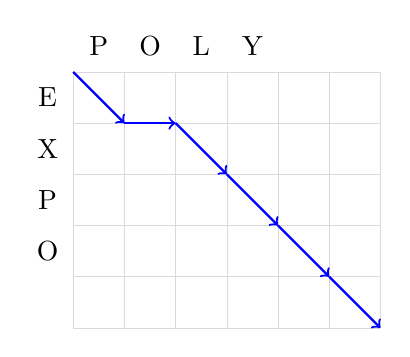
\begin{tikzpicture}[scale=0.65]
    \draw[step=1cm,gray!30,very thin] (0,0) grid (6,5);
    \node at (-0.5, 4.5) {E}; \node at (-0.5, 3.5) {X}; \node at (-0.5, 2.5) {P}; \node at (-0.5, 1.5) {O};
    \node at (0.5, 5.5) {P}; \node at (1.5, 5.5) {O}; \node at (2.5, 5.5) {L}; \node at (3.5, 5.5) {Y};
    \draw[->,thick,blue] (0,5) -- (1,4);
    \draw[->,thick,blue] (1,4) -- (2,4);
    \draw[->,thick,blue] (2,4) -- (3,3);
    \draw[->,thick,blue] (3,3) -- (4,2);
    \draw[->,thick,blue] (4,2) -- (5,1);
    \draw[->,thick,blue] (5,1) -- (6,0);
\end{tikzpicture}
\caption{编辑距离表格中的对齐路径（网格 DAG 中的最短路径）}
\label{fig:edit_grid}
\end{figure}

\begin{sidebarbox}{常见的子问题类型 (Common subproblems)}
寻找正确的子问题是动态规划的核心艺术。以下是四种最常见的子问题设定模式：
\begin{enumerate}
    \item \textbf{输入为 $x_1, \dots, x_n$ 单序列}：子问题为前缀 $x_1, \dots, x_i$（子问题数为 $O(n)$，如 LIS、背包问题）；
    \item \textbf{输入为两个序列 $x_1, \dots, x_n$ 与 $y_1, \dots, y_m$}：子问题为前缀对 $x_1, \dots, x_i$ 与 $y_1, \dots, y_j$（子问题数为 $O(mn)$，如编辑距离、最长公共子序列 LCS）；
    \item \textbf{输入为单序列且涉及区间合并}：子问题为区间切片 $x_i, \dots, x_j$（子问题数为 $O(n^2)$，如矩阵链乘、最优二叉搜索树）；
    \item \textbf{输入为有根树}：子问题为以 $u$ 为根的有根子树（子问题数为 $O(n)$，如树的最大独立集）。
\end{enumerate}
\end{sidebarbox}

\begin{sidebarbox}{人与小鼠：计算基因组学 (Of mice and men)}
人类 DNA 序列长达 30 亿个碱基对。在生物信息学中，比较基因序列、寻找物种进化同源基因（如小鼠与人类基因对比）的核心算法就是编辑距离的加权变体（Needleman-Wunsch 与 Smith-Waterman 算法），著名的序列比对工具 BLAST 亦深受其启发。
\end{sidebarbox}

\section{背包问题 (Knapsack)}

盗贼潜入房屋，背包总承重容量上限为 $W$ 磅。现有 $n$ 件物品，第 $i$ 件物品重量为 $w_i$，价值为 $v_i$。如何在不超重的前提下带走价值最高的物品组合？

\subsection{完全背包（物品可重复选取）}
定义子问题：$K(w)$ 为容量为 $w$ 的背包所能获得的最大价值。
递推状态转移方程：
\[
K(w) = \max_{i : w_i \le w} \{K(w - w_i) + v_i\}.
\]
算法从 $w = 1$ 到 $W$ 填一维数组，耗时 $O(nW)$。

\subsection{0-1 背包（每件物品最多选一件，不可重复）}
若物品不可重复，原一维状态无法记录物品是否已使用。增加维度：定义 $K(w, j)$ 为使用前 $j$ 件物品装入容量为 $w$ 的背包的最大价值。
对于第 $j$ 件物品，要么不选（价值为 $K(w, j - 1)$），要么选（价值为 $K(w - w_j, j - 1) + v_j$）：
\[
K(w, j) = \max \{K(w, j - 1),\; K(w - w_j, j - 1) + v_j\}.
\]
填补 $(W + 1) \times (n + 1)$ 的二维表格，总时间复杂度为 $O(nW)$（伪多项式时间）。

\begin{sidebarbox}{记忆化搜索 (Memoization)}
动态规划通常采用自底向上（Bottom-up）迭代填表的方式。另一种等价的实现是自顶向下（Top-down）递归并配合哈希表或查找表记录已计算过的子问题答案——这种技巧称为\textbf{记忆化 (Memoization)}。记忆化的优势在于它只会计算实际可达且需要的子问题状态，对于状态稀疏的问题极具优势。
\end{sidebarbox}

\section{矩阵链乘 (Chain matrix multiplication)}

计算四个矩阵相乘 $A \times B \times C \times D$（维度分别为 $50 \times 20, 20 \times 1, 1 \times 10, 10 \times 100$）。
虽然矩阵乘法满足结合律，但不同的括号加法顺序所需的标量乘法次数差异悬殊：
\begin{itemize}
    \item 方式一：$A \times ((B \times C) \times D)$ 需 120,200 次乘法；
    \item 方式二：$(A \times (B \times C)) \times D$ 需 60,200 次乘法；
    \item 方式三：$(A \times B) \times (C \times D)$ 仅需 \textbf{7,000 次乘法}！
\end{itemize}

给定矩阵序列 $A_1, \dots, A_n$（矩阵 $A_i$ 的维度为 $m_{i-1} \times m_i$），定义区间子问题：
令 $C(i, j)$ 为计算乘积矩阵链 $A_i \times \dots \times A_j$ 所需的最小乘法代价。
枚举最后一次矩阵乘法的分割点 $k$（$i \le k < j$）：
\[
C(i, j) = \min_{i \le k < j} \{C(i, k) + C(k + 1, j) + m_{i-1} \cdot m_k \cdot m_j\}.
\]
基础条件为 $C(i, i) = 0$。按照区间长度 $s = j - i$ 从小到大填表，总时间复杂度为 $O(n^3)$。

\section{最短路径进阶 (Shortest paths)}

\subsection{受限边数的最短可靠路径}
在不可靠网络中，每增加一跳都伴随着丢包风险。求从 $s$ 到 $t$ 且边数至多为 $k$ 边的最短路径。
定义子问题：$\text{dist}(v, i)$ 为从 $s$ 到 $v$ 恰好使用 $i$ 条边的最短路径长度：
\[
\text{dist}(v, i) = \min_{(u, v) \in E} \{\text{dist}(u, i - 1) + l(u, v)\}.
\]

\subsection{所有节点对最短路径 (Floyd-Warshall 算法)}
求解图中任意两点之间的最短路径。
定义子问题：令 $\text{dist}(i, j, k)$ 为从节点 $i$ 到节点 $j$、且所有中间节点编号均限制在 $\{1, 2, \dots, k\}$ 之内的最短路径长度。
递推状态转移：
\[
\text{dist}(i, j, k) = \min \{\text{dist}(i, j, k - 1),\; \text{dist}(i, k, k - 1) + \text{dist}(k, j, k - 1)\}.
\]
当 $k$ 从 1 递增至 $|V|$ 时，最终求得全源最短路径，总耗时为 $O(|V|^3)$。

\section{树上的独立集 (Independent sets in trees)}

图的独立集（Independent set）是指一个顶点子集 $S \subseteq V$，其中任意两点之间均没有边相连。在一般图上求最大独立集是 NP-完全难题，但在有根树上可以通过动态规划在线性时间 $O(|V|)$ 内求解！

定义子问题：令 $I(u)$ 为以节点 $u$ 为根的子树中的最大独立集大小。
\begin{itemize}
    \item 若独立集包含根节点 $u$，则 $u$ 的所有孩子节点都不能选，但可以自由选取 $u$ 的所有孙子节点；
    \item 若独立集不包含根节点 $u$，则可以自由选取 $u$ 的所有孩子节点。
\end{itemize}
因此得到树形 DP 状态转移方程：
\[
I(u) = \max \left\{ 1 + \sum_{w \text{ 为 } u \text{ 的孙子}} I(w),\; \sum_{v \text{ 为 } u \text{ 的孩子}} I(v) \right\}.
\]
从叶节点向根节点自底向上计算即可。

\newpage
\section*{习题 (Exercises)}
\addcontentsline{toc}{section}{习题}

\begin{exercise}{6.1}
给定包含 $n$ 个实数的数组 $a[1 \dots n]$，设计 $O(n)$ 动态规划算法求解最大连续子数组和（Kadane 算法）。
\end{exercise}

\begin{exercise}{6.2}
高速公路广告牌投放优化：在公路各里程桩点选址设立广告牌以最大化收益，受相邻广告牌距离不小于 $M$ 英里的约束。设计 $O(n)$ 动态规划算法。
\end{exercise}

\begin{exercise}{6.3}
找零钱问题（Yen 硬币系统）：给定面额 $v_1, \dots, v_n$ 与总金额 $v$，设计 $O(nv)$ 动态规划算法求凑出金额 $v$ 所需的最少硬币枚数。
\end{exercise}

\begin{exercise}{6.4}
字符串分词与字典匹配：给定无空格字符串与字典查询接口，设计 $O(n^2)$ 算法判断字符串是否可以被拆分为合法单词序列。
\end{exercise}

\begin{exercise}{6.5}
生物序列比对的 Pebble 棋盘博弈。
\end{exercise}

\begin{exercise}{6.6}
乘法优先级求值问题：给定布尔表达式与运算符真值表，设计 $O(n^3)$ 区间 DP 算法判断加括号能否使表达式计算结果为真。
\end{exercise}

\begin{exercise}{6.7}
最长公共子序列（LCS，Longest Common Subsequence）：设计 $O(mn)$ 算法求两个序列的最长公共子序列。
\end{exercise}

\begin{exercise}{6.8}
最长公共递增子序列（LCIS）：设计高效动态规划算法求两个数字序列的最长公共且严格递增的子序列。
\end{exercise}

\begin{exercise}{6.9}
切木棍的最小代价问题：长度为 $L$ 的木棍在若干指定标记点处切割，每次切割代价等于当前木棍长度，设计 $O(n^3)$ 区间 DP 求解最优切割次序。
\end{exercise}

\begin{exercise}{6.10}
抛硬币博弈赌注策略优化。
\end{exercise}

\begin{exercise}{6.11}
带界限的背包问题变体：每种物品有固定的供应数量上限 $c_i$。
\end{exercise}

\begin{exercise}{6.12}
双背包问题：盗贼有两个承重分别为 $W_1$ 和 $W_2$ 的背包，设计算法最大化装入两背包的物品总价值。
\end{exercise}

\begin{exercise}{6.13}
DNA 序列的局部最优局部对齐（Smith-Waterman 算法）。
\end{exercise}

\begin{exercise}{6.14}
无重复数字的子集和问题（Subset Sum）：设计 $O(nS)$ 算法判断是否存在和恰为 $S$ 的子集。
\end{exercise}

\begin{exercise}{6.15}
集合均分问题（Partition）：判断集合是否能被平分为元素之和相等的两个子集。
\end{exercise}

\begin{exercise}{6.16}
汇率连续兑换套利的最优序列选择。
\end{exercise}

\begin{exercise}{6.17}
矩阵链乘的自顶向下记忆化搜索与括号方案回溯重构。
\end{exercise}

\begin{exercise}{6.18}
二维网格上的最优路径行走（网格路径权值和最大化）。
\end{exercise}

\begin{exercise}{6.19}
包含通配符“?”与“*”的正则表达式模式匹配动态规划算法。
\end{exercise}

\begin{exercise}{6.20}
最优二叉搜索树（Optimal Binary Search Tree）：给定各关键字访问概率，设计 $O(n^3)$ 算法构建期望搜索代价最小的二叉搜索树。
\end{exercise}

\begin{exercise}{6.21}
树上的最大权顶点覆盖问题（Vertex Cover on Trees）。
\end{exercise}

\begin{exercise}{6.22}
多边形三角剖分的最小弦长代价和问题。
\end{exercise}

\begin{exercise}{6.23}
两台处理机的任务调度与完成时间（Makespan）最小化。
\end{exercise}

\begin{exercise}{6.24}
股票买卖最佳时机（包含交易冷冻期与最多交易 $k$ 次限制）。
\end{exercise}

\begin{exercise}{6.25}
最长回文子序列（Longest Palindromic Subsequence）：设计 $O(n^2)$ 区间动态规划算法。
\end{exercise}

\begin{exercise}{6.26}
对齐三个基因序列的三维编辑距离算法（$O(n^3)$ 状态空间）。
\end{exercise}

\begin{exercise}{6.27}
文本排版与两端对齐断行折行美化（TeX 排版折行算法核心原理）。
\end{exercise}

\begin{exercise}{6.28}
树上点权独立集的最大化（带权树形 DP）。
\end{exercise}

\begin{exercise}{6.29}
旅行商问题（TSP）在小规模下的状态压缩动态规划算法（Held-Karp 算法，$O(n^2 2^n)$）。
\end{exercise}

\begin{exercise}{6.30}
带负权边 DAG 上的所有节点对最短距离线性算法。
\end{exercise}
